\chapter{Evaluation}
\label{chapter:evaluation}

Kata Containers hardens the security of containerized environment by adding the extra layer of security with the micro VM. The added security features are enabled by the architectural change and new components of the environment. These components, such as the micro VM and hypervisor come with a price of degraded performance and computational overhead. Previous work, such as \cite{EverartsdeVelp2020} and \cite{Kumar2020} have examined the performance when compared Kata Containers against the native runtime runC, the most common OCI-compliant runtime. In these two papers, Kata Containers architecture design results in a performance decrease in IO throughput and overhead in memory and CPU utilization. However, the results in these papers are highly dependant on the underlying test environment. These tests do not consider the latest development and performance optimization of Kata Containers performance. In this paper, the system performance is evaluated in an environment simulating a telco edge cloud architecture and regular workload.

\textcolor{red}{Are there any expectations?}
\textcolor{red}{Results?}
\textcolor{red}{What the results mean?}

\section{Test architecture}
\label{section:test_architecture}

Telco applications are relying on high-performing and optimized computing. The ever-more increasing performance requirements from users add a great demand on the underlying infrastructure. Software and hardware based architectural changes to the edge cloud environment need to be carefully evaluated before implementing into the production as it might otherwise stall the performance and greatly decrease the performance for mobile network users.

The test environment, visualized in Figure \ref{fig:TestArchitectureCluster}, is a simple single-node cluster with one container. The main focus of the tests is to evaluate the impact of Kata Containers and the choice of hypervisor to I/O operations throughput and latency on various storage methods, such as Persistent Volume (PV), emptyDir, and hostPath. The full test combination matrix is described in Table \ref{table:TestMatrix}. The tests also measure CPU and memory overhead of Kata Containers architecture in general. The test cluster is hosted on K3s\cite{K3s} version 1.17.3, which is a lightweight version of Kubernetes supporting the identical API. K3s is Kubernetes distribution built for IoT and edge computing with lower footprint on memory and disk usage. K3s uses containerd as native container runtime engine. Due to compatibility issues, Kata Containers uses version XXX.

\begin{figure}[ht]
  \begin{center}
    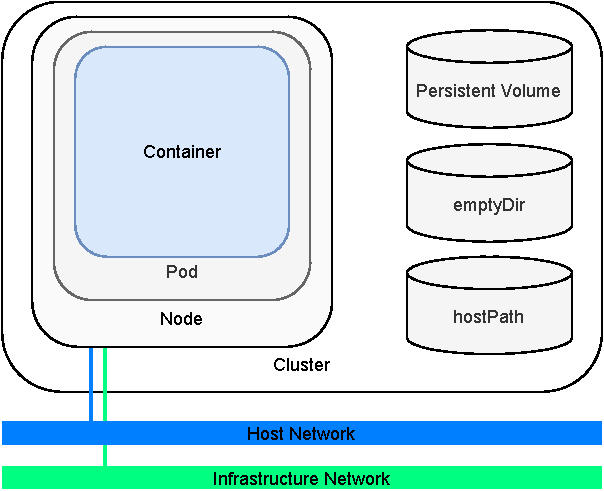
\includegraphics[width=12cm]{images/TestArchitectureClusterSimple.pdf}
    \caption{Kubernetes test cluster overview}
    \label{fig:TestArchitectureCluster}
  \end{center}
\end{figure}

\section{Methodology}

The tests of this thesis aim to measure the possible performance degradation of I/O operations and additional CPU and memory resource consumption due to the Kata Containers architecture. The test environment is hosted by a dedicated server which is built and tailored to support edge and far edge cloud deployments. The server includes Intel Xeon 6212U CPU with 24 cores and 48 threads with x86 architecture at 2.40 GHz clock-speed and 192GB of DDR4 memory at 2933 MHz clock-speed, which is shared to the cluster.

The performance tests run with Fio \cite{FIO}, an I/O performance tester with aim to simulate a variety of I/O workloads without resorting to writing a tailored test cases repeatedly. Fio supports a wide variety of test configurations such as multiple threads, block sizes, I/O sizes, and I/O patterns. In these thesis, the tests are time-based, where each tests runs for 30 seconds. The file size of each writable file is 2 GB. The Fio jobfile is described in Appendix \ref{appendix:fio_jobfile}. Each test is repeated three times, and the results are averaged. Table \ref{table:TestMatrix} describes the test combination matrix. In the tests each combination is sampled, resulting in 1200 different test scenarios. 

\begin{table}[ht]
\centering
\caption{Test combinations matrix}
\vspace{\baselineskip}
\begin{tabular}{| c | c | c | c | c |}
\hline
\textbf{Runtime} & \textbf{Jobs} & \textbf{Block size} & \textbf{I/O pattern} & \textbf{I/O device} \\ 
\hline
Bare metal & 1 & 512 & read & emptyDir (memory) \\
\hline
runC & 2 & 2048 & write & emptyDir (disk) \\ 
\hline
CLH & 3 & 8192 & randread & local (PV) \\
\hline
QEMU & & 16384 & randwrite & hostPath \\
\hline
QEMU VirtioFS & & 65536 & & \\
\hline
\end{tabular}
\label{table:TestMatrix}
\end{table}

The test matrix consists of five columns: runtime, jobs, block size, I/O pattern, and I/O device, Runtime of the tests refers to the container runtime or hypervisor. In the case of bare metal, the test is run on host without containerization. In bare metal test runs, the performance test is launched with CPU affinity to an isolated CPU with taskset\cite{taskset} command. Jobs refer to the number of concurrent clones. Each clone of job is spawned as an independent thread or process. Block size is the size in bytes for I/O units applying for reads and writes. I/O pattern has sequential and random pattern reads and writes. The I/O type is buffered. I/O device refers to the storage media used for test destination. EmptyDir is created on the container, whereas local Persistent Volume and hostPath are maintained by the host.

Fio test suite is wrapped inside a Docker image with a Linux OS Alpine\cite{Alpine}, which aims to deliver general purpose Linux with security, simplicity, and resource efficiency. The tests are deployed with Helm\cite{Helm}, a package manager for Kubernetes helping with deployment of applications. The Kubernetes Pods are deployed as Guaranteed Quality-of-Service with two CPUs and 18GB of memory to support the tests. However, each Kata Containers VM and runC container gets assigned with only 1 CPU. This restriction allows comparison of tests to bare metal tests, which are run on an isolated single CPU environment. The system performance, to measure CPU and memory overhead, is logged with Prometheus and Grafana.

\section{Results}

The tests are run one test at the time, and final results are averaged out of three tests. Fio provides a comprehensive catalog of parameters as test results, of which the most import ones are completion latency, I/OPS, and IO throughput. Completion latency describes the completion time in milliseconds for key percentile such as 50\% and 99.99\%. IOPS is the number of I/O operations per second. IO throughput or bandwidth in megabytes per second, is sum of block size multiplied with IOPS.

\subsection{I/O performance}






- Performance of root filesystem
	- Access fs of container
	- Overlay2 fs

- Access to mounted volumes in K8s
	- Create hostPath persistent volume
	- Attach
	- IO

- Attach empty dir to a container
	- Share fs between to containers in a same pod
	- RAM and disk
	- How this is possible?

\subsection{Storage performance}

- Access to mounted volumes in K8s \\
    - hostPath, emptyDir, local PV \\
	- Create persistent volume \\
	- Attach \\
	- IO

\subsection{CPU performance}

The architectural design of Kata Containers adds extra components to the system. Each of these components add overhead to the CPU performance via background processes. In the CPU performance tests, the main question was to measure the overhead and the need for extra cores in comparison to runC. The measurement of CPU performance was implemented by creating workloads and recording the performance with Prometheus. 

- CPU overhead of Kata
	- How many cores are needed when Kata is used?
	- From host perspective?
	- Measure
		- Create and delete workloads and record the CPU performance
			- Starting micro-VM might affect the CPU performance
			- Monitor with Prometheus

\subsection{Memory performance}

- Measuring performance of memory not important

- Memory overhead
	- How much the Kata adds to memory used?

\subsection{Network performance}

Networking
    - Evaluate performance \\
    - Two networks. What is the difference?
    - Access to storage not via network, unless NFS(?).

\section{Evaluation}